%     \noindent
%     \begin{minipage}{0.7\textwidth}    
%     \begin{definition}[Pushout \cite{barr1990category, overbeek2023graph}]
%         \label{def:cat:po}
%         % \begin{figure}[htbp] 
%         %     \centering
%         %         % \begin{tikzpicture}
%         %         %     \node (i) at (0,0) {A};
%         %         %     \node (r) at (1,1) {B};
%         %         %     \node (c) at (1,-1) {C};
%         %         %     \node (h) at (2,0) {D};
%         %         %     % \node () at (1,-1) {\( \Delta \)};
%         %         %     \draw[->]  (i) -- (r) node [midway,left] {$ \alpha $};
%         %         %     \draw[->] (c) -- (h) node [midway,left] {$ \alpha' $};
%         %         %     \draw[->] (r) -- (h) node[midway, left] {$ \beta' $};
%         %         %     \draw[->] (i) -- (c) node[midway, left] {$ \beta $};
%         %         %     \node (d') at (4,0) {E};
%         %         %     \draw[->] (c) -- (d') node [midway,below]{$ \gamma $};
%         %         %     \draw[->] (r) -- (d') node [midway,above]{$ \gamma' $};
%         %         %     \draw[->,dashed] (h) -- (d') node [midway]{$ \delta $};
%         %         % \end{tikzpicture}
%         %         \caption{pushout of span \( (\alpha, \beta) \)}
%         %         \label{diag:def_pbpo_po}
%         % \end{figure}
%         A \textbf{pushout} of a span \( B \overset{\alpha}{\leftarrow} A \overset{\beta}{\rightarrow} C \) is defined as a cospan \( B \overset{\beta'}{\rightarrow} D \overset{\alpha'}{\leftarrow} C \) such that 
%         \begin{itemize}
%             \item \( \alpha \star \beta' = \beta \star \alpha' \);
%             \item for every cospan \( B \overset{\gamma'}{\rightarrow} E \overset{\gamma}{\leftarrow} C \), if \( \alpha \star \gamma' = \beta \star \gamma \) holds, then there exists a unique morphism \(\delta : D \to E\) such that \( \gamma' = \beta' \star \delta \) and \( \gamma = \alpha' \star \delta \). 
%         \end{itemize}
%     \end{definition} 
% \end{minipage}
% \begin{minipage}{0.299\textwidth}
%     \resizebox{0.9\textwidth}{!}{
%                \begin{tikzpicture}
%                     \node (i) at (0,0) {A};
%                     \node (r) at (1,1) {B};
%                     \node (c) at (1,-1) {C};
%                     \node (h) at (2,0) {D};
%                     % \node () at (1,-1) {\( \Delta \)};
%                     \draw[->]  (i) -- (r) node [midway,left] {$ \alpha $};
%                     \draw[->] (c) -- (h) node [midway,left] {$ \alpha' $};
%                     \draw[->] (r) -- (h) node[midway, left] {$ \beta' $};
%                     \draw[->] (i) -- (c) node[midway, left] {$ \beta $};
%                     \node (d') at (4,0) {E};
%                     \draw[->] (c) -- (d') node [midway,below]{$ \gamma $};
%                     \draw[->] (r) -- (d') node [midway,above]{$ \gamma' $};
%                     \draw[->,dashed] (h) -- (d') node [midway]{$ \delta $};
%                 \end{tikzpicture}
%     }
% \end{minipage}
% The diagram involving \(\alpha\), \(\beta\), \(\alpha'\), and \(\beta'\) is referred to as the \textbf{pushout square}, \(D\) as the \textbf{pushout object}, and the existence of the unique morphism is known as the \textbf{universal mapping property of the pushout}.
\begin{definition}[Pushout \cite{barr1990category}]
    \label{def:cat:po}
    \ \newline
\noindent
\begin{minipage}{0.7\textwidth}  
    A \textbf{pushout} of a span \( B \overset{\alpha}{\leftarrow} A \overset{\beta}{\rightarrow} C \), as shown on the right, is defined as a cospan \( B \overset{\beta'}{\rightarrow} D \overset{\alpha'}{\leftarrow} C \) such that \( \alpha \star \beta' = \beta \star \alpha' \), and for every cospan \( B \overset{\gamma'}{\rightarrow} E \overset{\gamma}{\leftarrow} C \), if \( \alpha \star \gamma' = \beta \star \gamma \) holds, then there exists a unique morphism \(\delta : D \to E\) such that \( \gamma' = \beta' \star \delta \) and \( \gamma = \alpha' \star \delta \).
\end{minipage}
\hfill
\begin{minipage}{0.299\textwidth}
    \hfill
\resizebox{0.9\textwidth}{!}{
           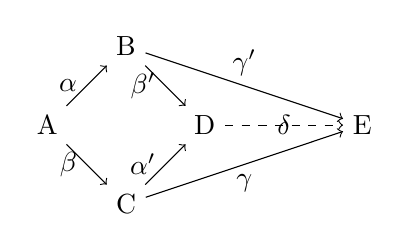
\begin{tikzpicture}
                \node (i) at (0,0) {A};
                \node (r) at (1,1) {B};
                \node (c) at (1,-1) {C};
                \node (h) at (2,0) {D};
                % \node () at (1,-1) {\( \Delta \)};
                \draw[->]  (i) -- (r) node [midway,left] {$ \alpha $};
                \draw[->] (c) -- (h) node [midway,left] {$ \alpha' $};
                \draw[->] (r) -- (h) node[midway, left] {$ \beta' $};
                \draw[->] (i) -- (c) node[midway, left] {$ \beta $};
                \node (d') at (4,0) {E};
                \draw[->] (c) -- (d') node [midway,below]{$ \gamma $};
                \draw[->] (r) -- (d') node [midway,above]{$ \gamma' $};
                \draw[->,dashed] (h) -- (d') node [midway]{$ \delta $};
            \end{tikzpicture}
}
\end{minipage}
The diagram involving \(\alpha\), \(\beta\), \(\alpha'\), and \(\beta'\) is referred to as the \textbf{pushout square}, \(D\) as the \textbf{pushout object}, and the existence of the unique morphism is known as the \textbf{universal mapping property of the pushout}.
\end{definition} 
